%%%FTK
\section{Fast Tracker}

The Fast TracKer (FTK) system was foreseen as a significant upgrade for the TDAQ system of ATLAS by providing hardware-based tracking information directly to the HLT.
As discussed in Section 3.3, although the L1 trigger and HLT perform exceptionally in selecting physics events and reducing the event rate, this implementation does have its limitations.
Currently, the HLT receives the "hits" information recorded by the ID, essentially points in space, and conducts tracking calculations within the ROIs determined by the L1 trigger.
Tracking calculations in the HLT software are demanding and slow, leading to restrictions on the size and number of ROIs. 
The ROI approach also resulted in notable inefficiencies in jet finding, due to discrepancies between the online and offline strategies~\cite{TAMSETT2013253}~\cite{Aad2016}.
A solution is to use specialized hardware for this task, which is the primary goal of the FTK system. FTK will be positioned between the L1 trigger and HLT, offering tracking information for all events that pass the L1 trigger across the entire detector and supplying this data to the HLT.

The FTK system consists of various types of boards and components, with details provided in Figure~\ref{fig:ftk_overview} and Table~\ref{table:ftk_overview}. The Input Mezzanines (IM) receive data directly from the Level 1 trigger (the RODs). There are a total of 12 layers from the Inner Detector: four double SCT layers, three Pixel layers, and one IBL.
Clustering is applied to the hits from these layers to reduce data flow. The clustered data is then sent to the Data Formatter (DF) system.
The DF system divides the data, sending eight layers (five from the SCT and three from the Pixel) to the main Processing Units (PU) and the remaining four layers (three SCT and one IBL) to the Second Stage Boards (SSB).

\begin{figure}[ht]
  \centering
  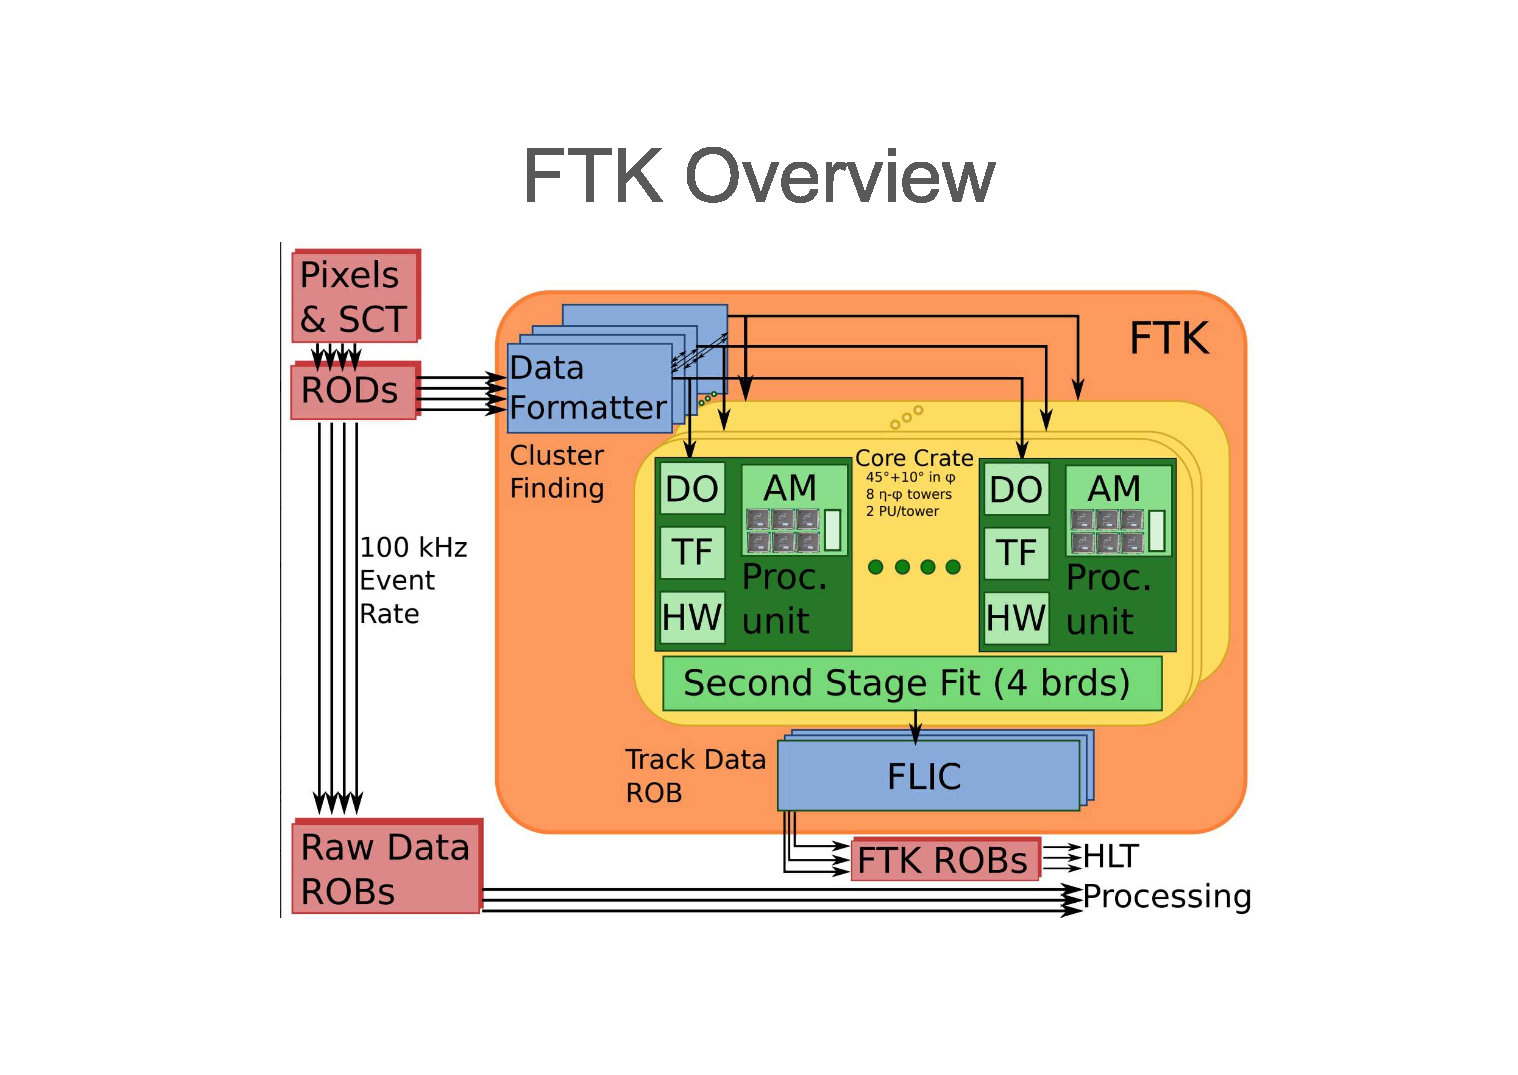
\includegraphics[width=0.95\textwidth]{figures/ftk/ftk_overview.pdf}
  \caption{Overview of the FTK system.}
  \label{fig:ftk_overview}
\end{figure}

\begin{table}[ht]
\centering
\resizebox{0.95\textwidth}{!}{%
\begin{tabular}{llllr}
\hline
\textbf{Module} & \textbf{Function} & \textbf{Type} & \textbf{Number} \\
\hline
\hline
IM & Input Mezzanine & Cluster Pixel and SCT hits, format module data & Mezzanine & 128 \\\hline
DF & Data Formatter & Transport and duplicate module hit data to \(\eta\)-\(\phi\) towers & ATCA & 32 \\\hline
AUX & Auxiliary Card & Transport coarse-resolution 8-layer hit data to AMB & VME & 128 \\\hline
AMB & AM Board & Transport hit data to AM & VME & 128 \\
AM & Associative Memory & Match hits to patterns & ASIC & 8192 \\
AUX & Auxiliary Card & Evaluate track candidates in matched patterns & VME & 128 \\\hline
SSB & Second Stage Board & Add remaining hits to 8-layer tracks, fit, remove overlaps & VME & 32 \\\hline
FLIC & HLT Interface Board & Interface to ATLAS readout & ATCA & 2 \\
\hline
\end{tabular}%
}
\caption{Overview of the FTK system in the order in which the data are processed. 
The AUX appears in the table twice because of its dual functions \cite{Aad_2021}.}
\label{table:ftk_overview}
\end{table}

The main Processing Units are made up of two boards: the Associated Memory Board (AMB) and the Auxiliary Board (AUX), with the AUX serving as a rear transmission module. The AMB is essential to the FTK system. To construct tracks rapidly, billions of precomputed tracks are stored in a large memory bank. These track patterns are then matched to the incoming hit coordinates using massive parallel processing. Each AMB can match eight million patterns in parallel to the incoming hit data.

The Auxiliary Board (AUX) communicates with its corresponding Associated Memory Board (AMB) via the VME backplane, performing a range of functions. Its principal duty involves eight-layer track fitting. The procedure is as follows:
\begin{itemize}
    \item Input data from the DF is forwarded to the AMB.
    \item The AMB, after matching patterns, returns them to the AUX.
    \item Utilizing these patterns, the AUX conducts a fit to assess their quality, allowing tracks to be missing a hit on one layer -- these are termed \textit{majority tracks} -- to boost efficiency.
    \item Moreover, the AUX undertakes the removal of duplicates among the eight-layer track candidates.
    \item Valid eight-layer tracks are then forwarded to the Second Stage Boards (SSB).
\end{itemize}

The Second Stage Board (SSB) system includes 32 boards, each responsible for managing tracks from four PUs. The SSB integrates these eight-layer tracks with hit data for the four additional layers from the corresponding DF, to assemble 12-layer tracks. This process involves:
\begin{itemize}
    \item Extrapolating the eight-layer track into the missing layers.
    \item Using hits near the extrapolated coordinates to fit full 12-layer tracks.
\end{itemize}
Like in the first stage, it is possible for tracks to be missing a hit in one of the new layers. After fitting, tracks undergo a global duplicate check before being forwarded to the FTK Level2 Interface Crate (FLIC). SSBs are paired to cover the entire detector range, with pairs linked in a ring to manage overlap.

The FTK Level2 Interface Crate (FLIC) is the last element in the FTK system, serving two primary purposes:
\begin{itemize}
    \item It merges the 12-layer track data from the 32 SSBs.
    \item It formats the consolidated data so that it can be interpreted by the Read Out System (ROS).
\end{itemize}

\subsection{Second Stage Board}

The Second Stage Boards (SSBs), designed and manufactured at the University of Illinois, perform three critical functions (see Figure~\ref{fig:ssb_board}):
\begin{itemize}
    \item Extrapolating incoming eight-layer tracks to include the missing layers,
    \item Fitting these extrapolations to form 12-layer tracks,
    \item Removing any duplicates found across the detector.
\end{itemize}
The hardware of the SSBs includes five Field-Programmable Gate Arrays (FPGAs) that require firmware. Four of these FPGAs, designated as the EXTF FPGAs, are dedicated to the tasks of extrapolation and track fitting. The fifth FPGA, known as the Hit Warrior (HW) FPGA, is tasked with duplicate removal. Furthermore, the SSBs are equipped with a substantial amount of Reduced Latency Dynamic Random-Access Memory (RLDRAM) for storing the constants necessary for extrapolation and track fitting calculations.
The layout and the dataflow through the SSB are shown in Figure~\ref{fig:ssb_diagram}.

\begin{figure}[ht]
  \centering
  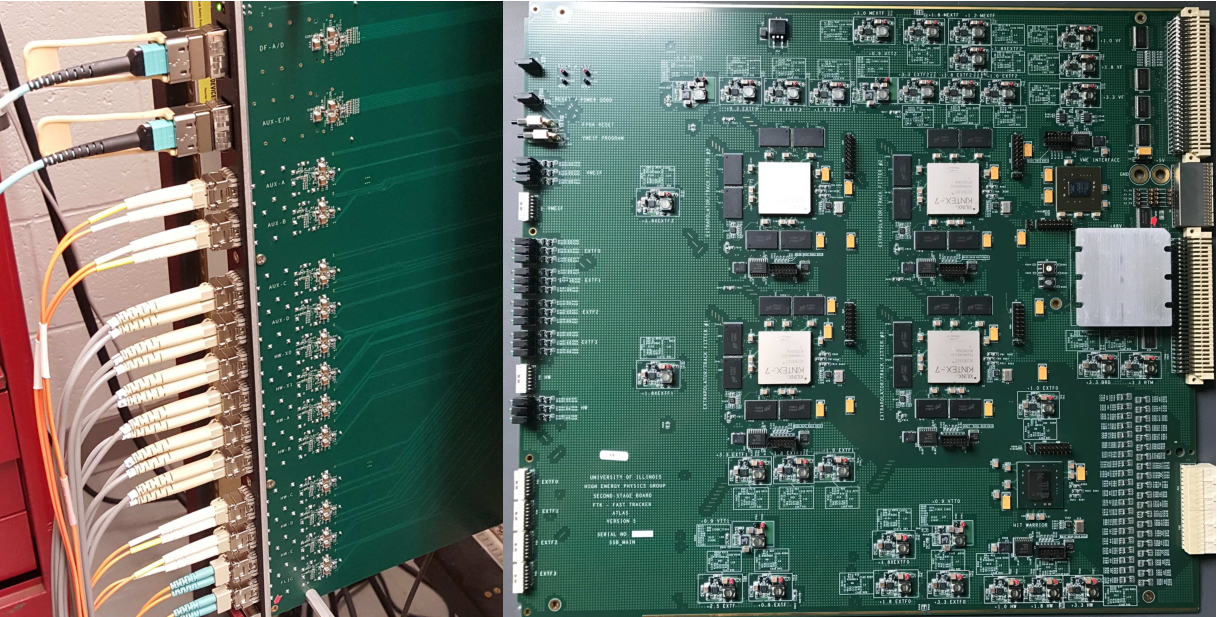
\includegraphics[width=0.75\textwidth]{figures/ftk/ssb_board.pdf}
  \caption{The physical Second Stage Boards~\cite{Aad_2021}.}
  \label{fig:ssb_board}
\end{figure}

\begin{figure}[ht]
  \centering
  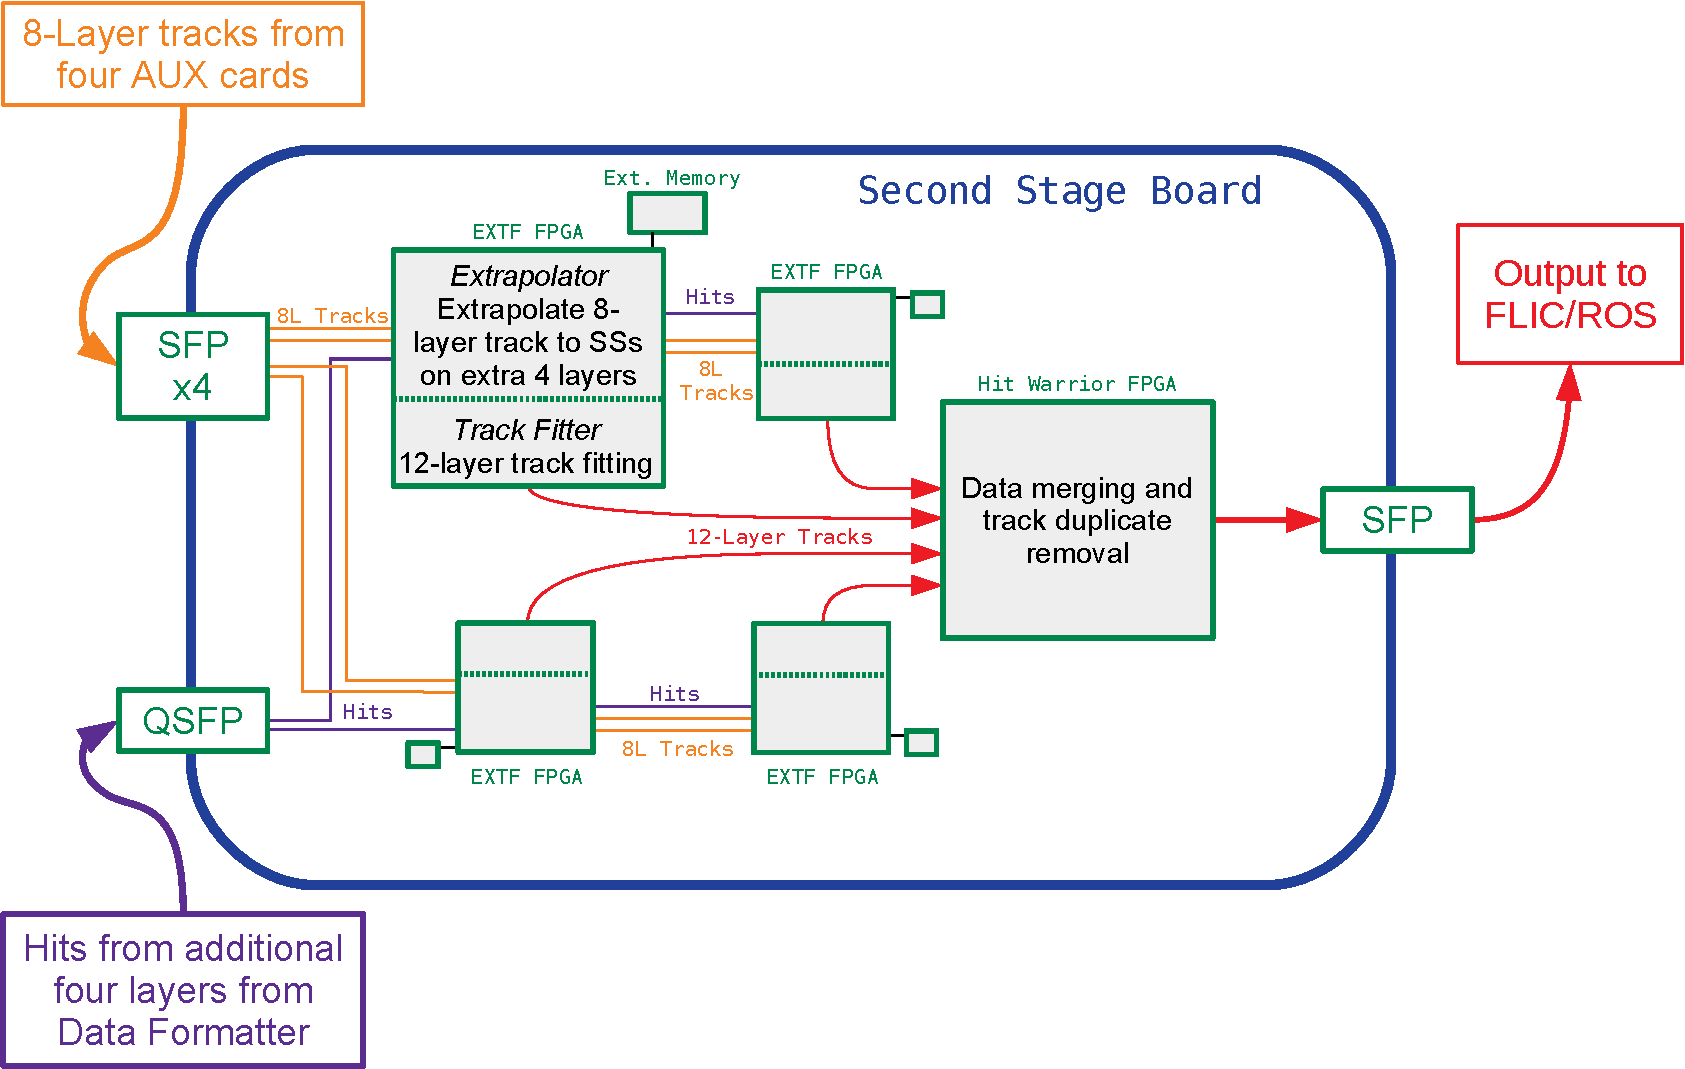
\includegraphics[width=0.75\textwidth]{figures/ftk/ssb_diagram.pdf}
  \caption{Diagram of the dataflow through the Second Stage Board~\cite{Aad_2021}.}
  \label{fig:ssb_diagram}
\end{figure}

The core functionality of the EXTF FPGA is allocated to the Extrapolator (EXP), which oversees the extrapolation process, and the Track Fitter (TF), focused on the fitting of the resulting 12-layer tracks. For a thorough exploration of these firmware aspects, see Markus Atkinson's PhD thesis \cite{Atkinson2019}.

\subsection{Hit Warrior FPGA}
The Hit Warrior FPGA on the SSB serves two key roles. Its main job is to eliminate duplicate tracks. Its second role involves merging data. Each SSB houses four EXTF FPGAs, and the Hit Warrior FPGA collects all their output. This output is then scanned for any duplicates, combined into a single large output packet, and forwarded to the FLIC.
The top-level diagram of the Hit Warrior firmware design is depicted in Figure~\ref{fig:hw_top_diagram}. In the diagram, the Sync Engine module synchronizes the four incoming EXTF streams. The Hit Warrior module is the logic component that performs the comparison and duplicate removal tasks. Additionally, Spy Buffers are utilized for monitoring purposes. More details on the Hit Warrior module follow.

\begin{figure}[ht]
  \centering
  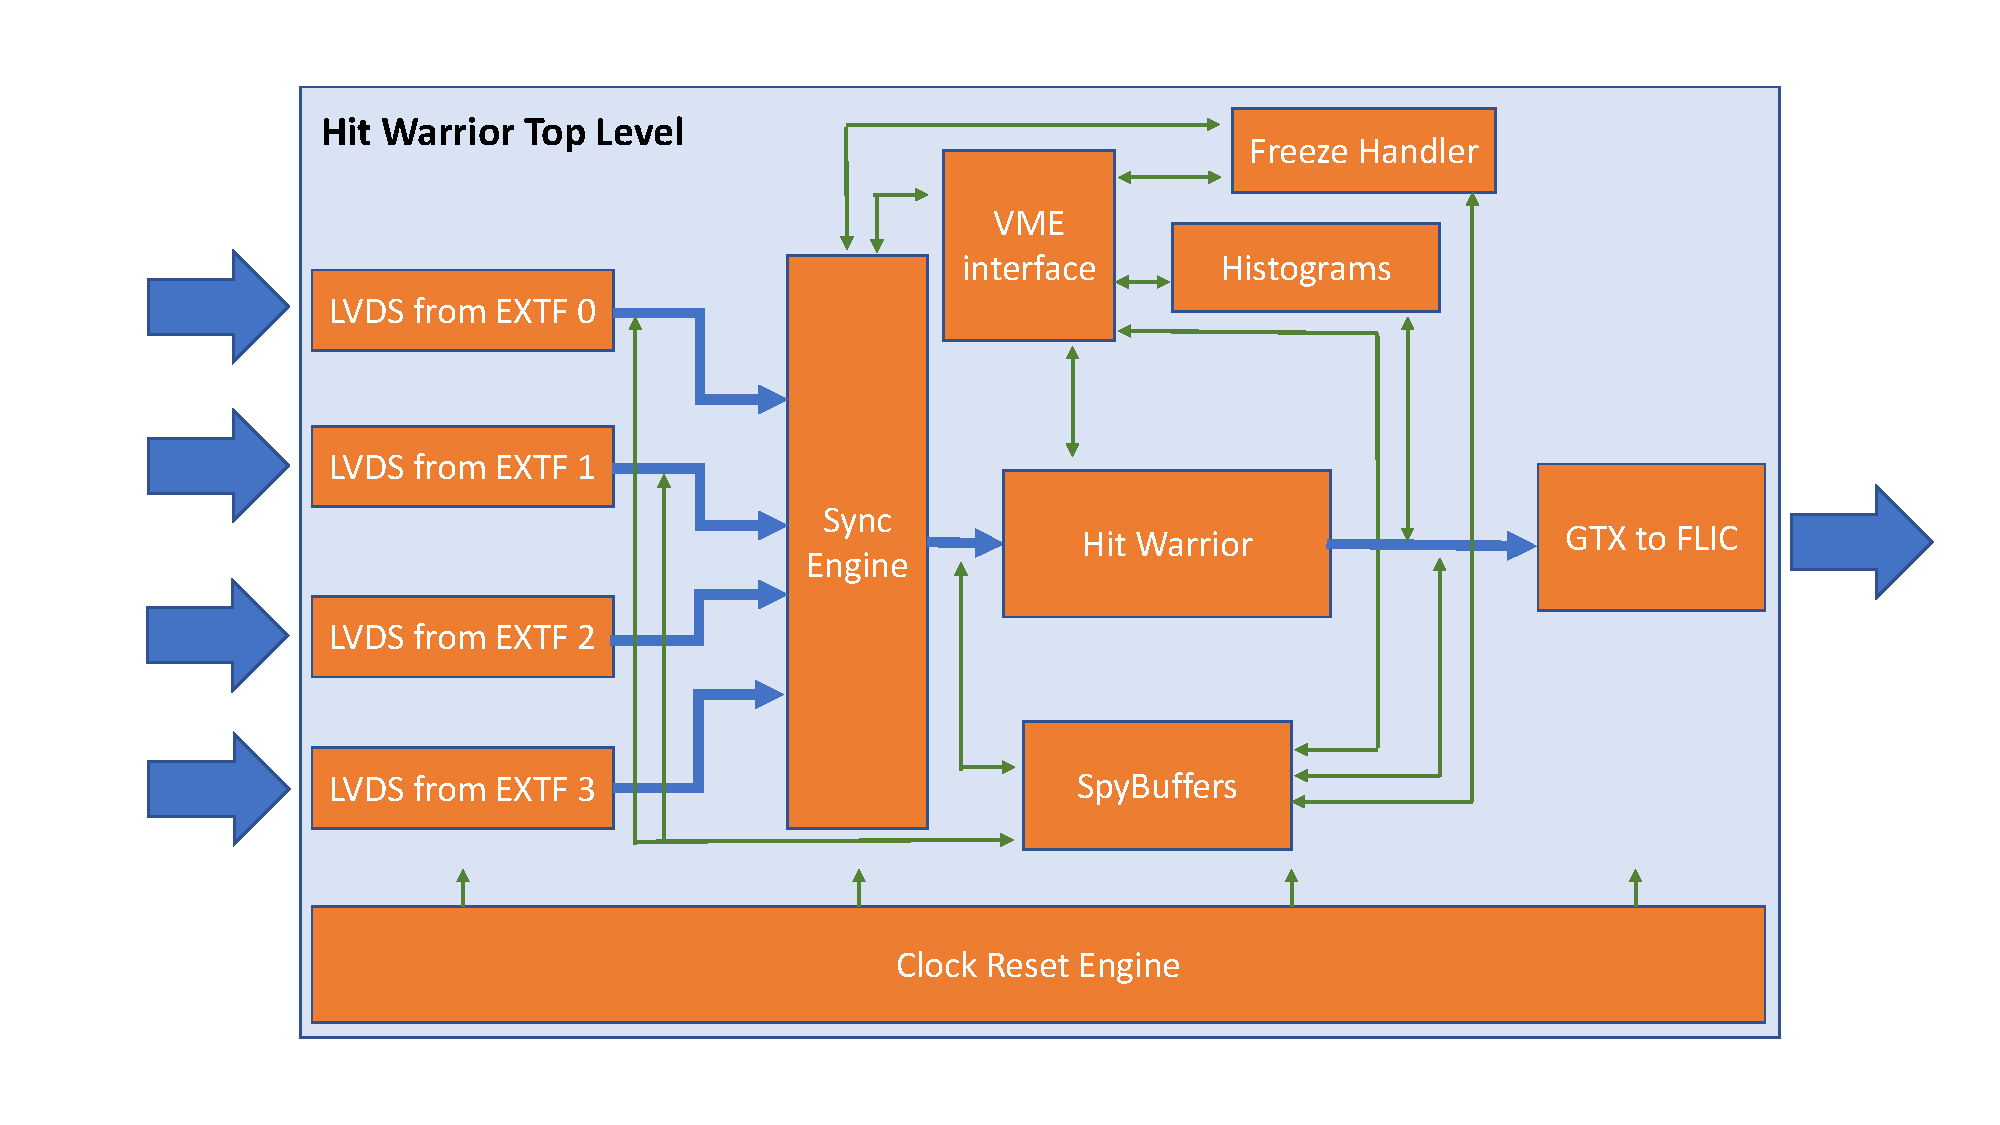
\includegraphics[width=0.75\textwidth]{figures/ftk/hw_top_diagram.pdf}
  \caption{Diagram of the Hit Warrior firmware~\cite{Aad_2021}.}
  \label{fig:hw_top_diagram}
\end{figure}

The Track Parser functions as the first component of the Hit Warrior module, where it examines the data to identify the start of track packets. These packets always start with the keyword ``BDA'' and consist of 28 words. Each track is distributed throughout the FPGA to enable parallel processing of track comparisons. Tracks are processed sequentially, one after another, which makes it practical to use a track counter. The specific processing path for each track depends on this counter. However, the overarching strategy ensures that each new track is compared with all previously received tracks simultaneously. By the time the final track is processed, all necessary track comparisons have been completed.

The first and simplest component to understand in this context is the RAW FIFO (First In, First Out). This acts as an internal storage or buffer for all the tracks corresponding to the current event, storing them in the exact order they were received.
The layout is illustrated in Figure \ref{fig:hw_fifo}.

\begin{figure}[ht]
  \centering
  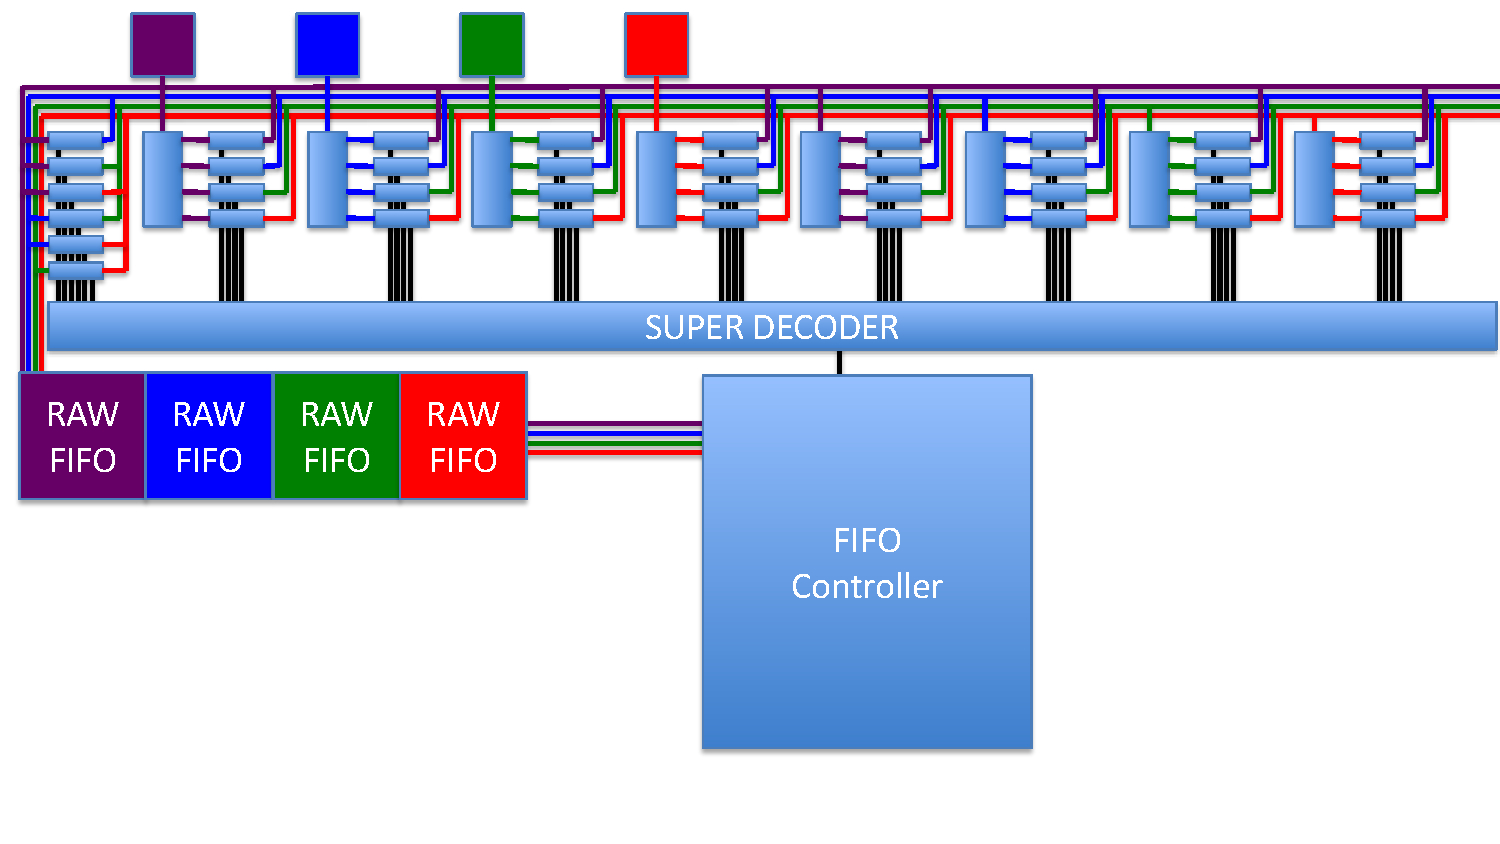
\includegraphics[width=0.75\textwidth]{figures/ftk/hw_fifo.pdf}
  \caption{Hit Warrior FIFO Diagram}
  \label{fig:hw_fifo}
\end{figure}

Tracks are also sent to units called Comparators. The total number of Comparators is limited by available resources, which in turn sets a maximum on the number of tracks that can be effectively compared for an event. Each Comparator is equipped with a small piece of RAM (Random Access Memory) capable of holding a single track packet. Furthermore, each Comparator is directly connected to the stream of incoming tracks, allowing it to receive and compare new track data as it arrives.

%%%Comparators
The comparator conducts comparisons between two tracks on a word-to-word basis to identify matches. Each track packet contains 28 words, comprising 12 for the Track Header and 16 for the hit list. These 16 words are distributed across 12 layers. A match requires at least eight layers to be identical, a criterion determined through simulation to ensure maximum efficiency. For 2D pixel layers, both coordinates must match.

When matches are detected, a selection criterion decides the optimal track. Tracks with the same number of layers are evaluated on their \(\chi^2\) values to select the best one. If the layer count varies, the track with the greater number of layers is chosen. The selection scheme is outlined in the Table~\ref{table:track_selection_scheme}.

\begin{table}[ht]
\centering
\resizebox{0.6\textwidth}{!}{%
\begin{tabular}{ccc}
\hline
\textbf{Track 1} & \textbf{Track 2} & \textbf{Decision} \\
\hline
Nominal & Nominal & Select Track with lowest \(\chi^2\) \\
Nominal & Majority & Select Nominal Track \\
Majority & Majority & Select Track with lowest \(\chi^2\) \\
\hline
\end{tabular}%
}
\caption{Selection scheme for matching tracks.}
\label{table:track_selection_scheme}
\end{table}

After each track is compared, the outcome is forwarded to the Decoder, which logs the results of all track comparisons. Each comparator can issue one of four possible outcomes, encoded as two bits: \textit{idle}, \textit{no match}, \textit{delete RAM}, and \textit{delete Stream}. The Decoder synthesizes these outcomes with the current track count and the comparator's index to generate a ``copy vector.'' This vector is essential for managing the write process to the CUT FIFO.

Once every track for the event has been examined and the copy vector is complete, the RAW FIFO's content is moved. This FIFO contains a copy of every track. This data is then transferred to a second FIFO, named the CUT FIFO, guided by the copy vector to ensure only the valid tracks are preserved. This arrangement allows for the removal of gaps in the data by excluding the tracks as dictated by the copy vector.

\begin{table}[ht]
\centering
\begin{tabular}{ll}
\hline
\textbf{Comparator Output} & \textbf{Meaning} \\
\hline
Idle & No operation \\
No Match & No duplicate found \\
Delete RAM & Remove track from RAM \\
Delete Stream & Remove track from incoming stream \\
\hline
\end{tabular}
\caption{Comparator Results and Their Meanings}
\label{table:comparator_results}
\end{table}

The CUT FIFO then serves as the final repository for the processed tracks, ensuring that only the relevant tracks are stored for further processing.
The decoder, using comparator flags, the index number of each comparator, and the track counter, identifies tracks for deletion. For instance, comparator M can only eliminate track M stored in its RAM or the track currently indexed by the track counter. Each processed track is compared in parallel to all prior ones. In each comparison round, any previous track might be marked for deletion by the incoming track. After each round, the decoder updates the copy vector to record any tracks flagged for removal. When the last track of the event has been compared, the final version of the copy vector is used to regulate the transfer of data from the RAW FIFO to the CUT FIFO, ensuring only the required tracks are retained.

It became apparent later in development that the prototype Hit Warrior firmware couldn’t keep up with the required processing speed. To address this, the system was adapted to process multiple streams in parallel. The Parallel Hit Warrior operates much like the original but at quadruple the speed by handling four streams simultaneously. This choice is aligned with the four EXTF FPGAs on each SSB. Therefore four tracks are inputted into four separate comparators. These comparators have been adapted to match a track in RAM against four incoming stream tracks at the same time. Additionally, a new component, the Cross Comparator, was introduced to compare all six pairings among the four stream tracks.
The layout of the Parallel Hit Warrior is shown in Figure \ref{fig:hw_layout}, and the details of the comparator are revealed in Figure \ref{fig:hw_details}.

\begin{figure}[ht]
  \centering
  \begin{subfigure}[b]{0.5\textwidth}
    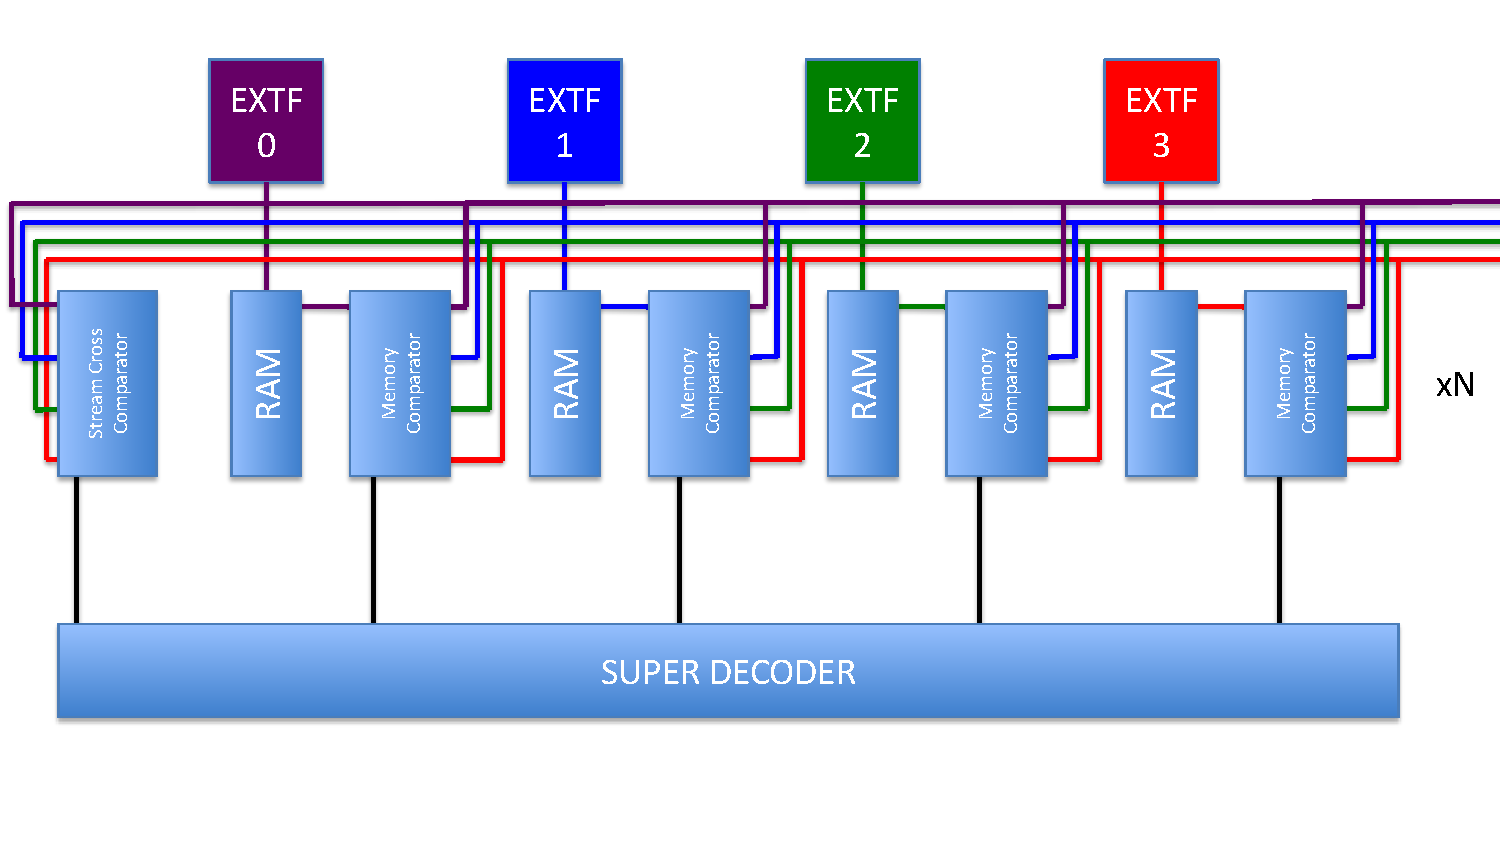
\includegraphics[width=\textwidth]{figures/ftk/hw_layout.pdf}
    \caption{Hit Warrior Layout}
    \label{fig:hw_layout}
  \end{subfigure}%
  \hfill
  \begin{subfigure}[b]{0.5\textwidth}
    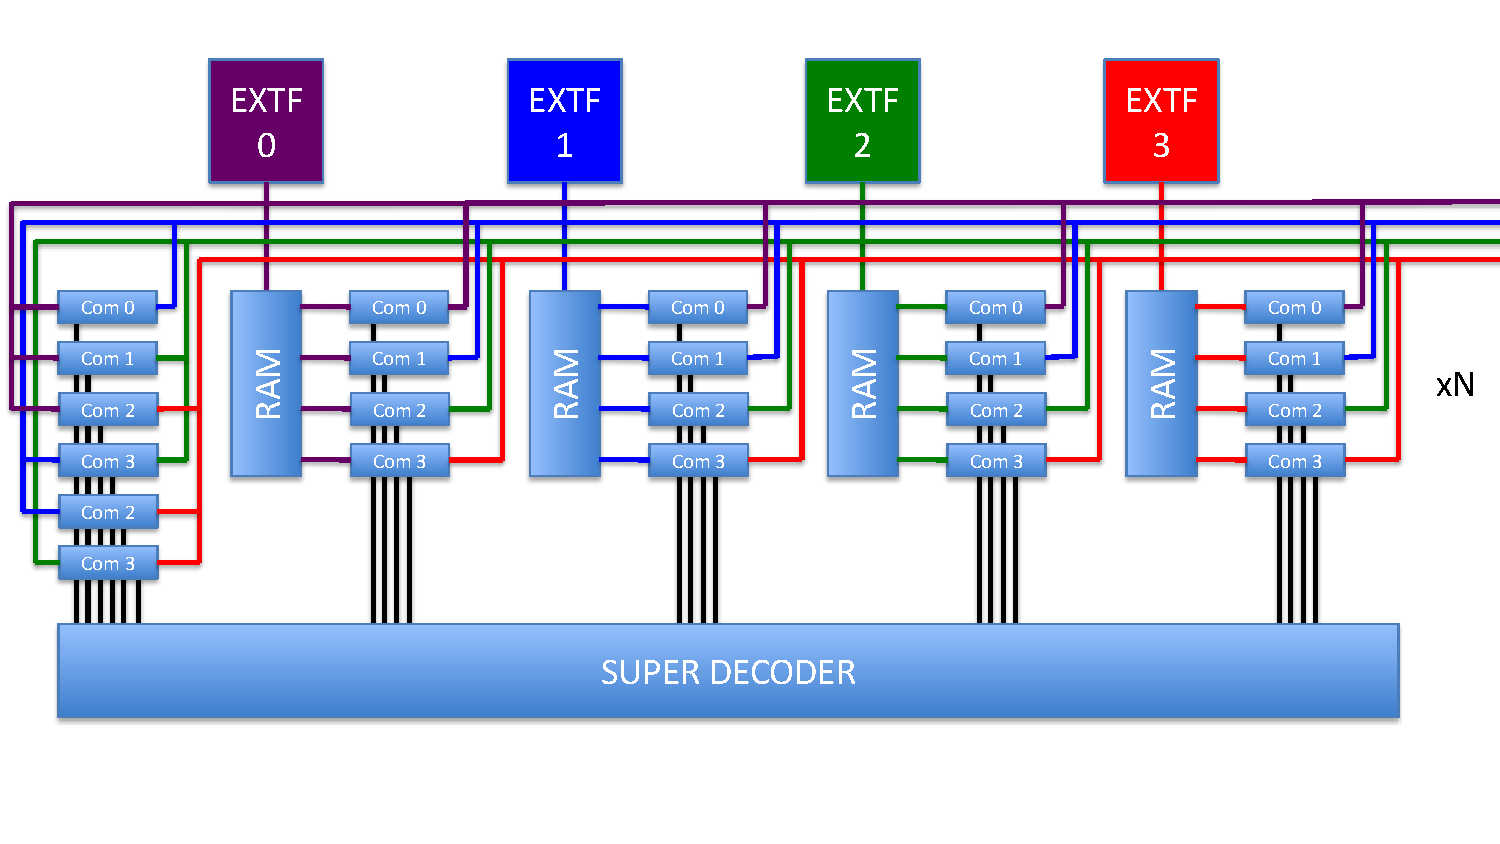
\includegraphics[width=\textwidth]{figures/ftk/hw_details.pdf}
    \caption{Hit Warrior Details}
    \label{fig:hw_details}
  \end{subfigure}
  \caption{Hit Warrior System Components}
  \label{fig:hit_warrior}
\end{figure}

%Spybuffer
The firmware design for the HitWarrior FPGA utilizes circular buffers, known as Spy Buffers, to capture data as it moves through the system, alongside the capability to read out monitoring registers. It also allows for the freezing of monitoring data in the event of errors to aid in debugging. Furthermore, these buffers store synchronized monitoring information and compile histograms of monitoring data. While this firmware design is broadly applied across various components of the FTK system, including the design of synchronization blocks, the SSB version is tailored for the HitWarrior FPGA to meet specific design needs and to accommodate the architecture of the FPGA chip.
As shown in Figure~\ref{fig:hw_top_diagram}, the Spy Buffers monitor the four parallel streams from the EXTF FPGAs, and the output of the Hit Warrior module before sending it to the FLIC.

%my job

My role in the development of the SSB involved updating the firmware for the Hit Warrior FPGA, focusing on parallelizing the prototype Hit Warrior firmware and implementing the Spy Buffers. 
I was deeply involved, often as the sole representative for the SSB, in its commissioning and integration into the ATLAS trigger system. This required extensive hours in the ATLAS control rooms and the underground facilities where the FTK system is installed.




